\documentclass[11pt]{amsart}

\usepackage{amsmath,amssymb,amsthm,mathtools}
\usepackage[margin=1.15in]{geometry}
\usepackage{enumitem}
\usepackage{cite}
\usepackage{tikz}
\usetikzlibrary{calc}
\usepackage[hidelinks]{hyperref}

\hypersetup{
  pdftitle={Strong terminal failures of log-concavity in independence polynomials of subcubic trees},
  pdfauthor={Knowledge Sense},
  pdfsubject={Independence polynomials of trees},
  pdfkeywords={independence polynomial, log-concavity, tree, maximum degree}
}

\newtheorem{theorem}{Theorem}[section]
\newtheorem{lemma}[theorem]{Lemma}
\newtheorem{proposition}[theorem]{Proposition}
\newtheorem{corollary}[theorem]{Corollary}
\theoremstyle{definition}
\newtheorem{definition}[theorem]{Definition}
\theoremstyle{remark}
\newtheorem{remark}[theorem]{Remark}

\numberwithin{equation}{section}
\setlength{\emergencystretch}{1.5em}

\newcommand{\cI}{\mathcal{I}}
\newcommand{\cX}{\mathcal{X}}
\newcommand{\cA}{\mathcal{A}}
\newcommand{\R}{\mathsf{R}}
\newcommand{\coef}[2]{[x^{#1}]#2}
\newcommand{\cs}{\circledast}

\begin{document}

\title[Terminal failures of log-concavity in subcubic trees]{Strong terminal failures of log-concavity in independence polynomials of subcubic trees}

\author{Knowledge Sense}
\address{Knowledge Sense}
\email{math@knowledgesense.jp}

\date{12 October 2026}

\subjclass[2020]{Primary 05C31; Secondary 05C05, 05C69, 05A20}

\keywords{Independence polynomial, independent set sequence, log-concavity, tree, maximum degree}

\begin{abstract}
For a graph $G$ let $s_k(G)$ be the number of independent sets of size $k$ in $G$, and let $\alpha(G)$ be its independence number. We show that for all integers $r,H\ge 1$ there is an explicitly constructed tree $T$ of maximum degree at most three, on at most ${1200(r+1)^4\bigl(r+1+\lceil\log_2(H+1)\rceil\bigr)}$ vertices, such that
\[
s_{\alpha-j-1}(T)\,s_{\alpha-j+1}(T)>H\,s_{\alpha-j}(T)^2\qquad(1\le j\le r),\quad \alpha=\alpha(T).
\]
Thus log-concavity of the independent set sequence fails at each of the $r$ last possible positions $\alpha-1,\dots,\alpha-r$, and each failure has ratio larger than $H$. In the infinite families with proved consecutive failures, runs ending at $\alpha-1$ have length at most three, longer runs do not contain the positions next to $\alpha$, and the maximum degree is unbounded. Our tree consists of paths whose vertices carry rooted blocks of different weights. The blocks come from a subcubic recursion in which a block with $O(p\log a)$ vertices has, after deletion of its root, between $a^p$ and $a^pe^{2p/a}$ maximum independent sets. The highest coefficients are compared, up to a factor $2^{r+4}$, with an explicit model whose $j$-th coefficient is a binomial coefficient $\binom{r+1}{j}$ times a power of a large integer $a$, with exponent quadratic in $j$ and leading term $j^2$. Degree three is the smallest possible degree bound, and for fixed $r$ the growth of the number of vertices as a multiple of $\log H$, as $H\to\infty$, cannot be improved.
\end{abstract}

\maketitle

\section{Introduction}

For a finite simple graph $G$ let $s_k(G)$ denote the number of independent sets of size $k$ in $G$, let $\alpha(G)$ be the independence number, and let
\[
I(G;x)=\sum_{k=0}^{\alpha(G)}s_k(G)x^k
\]
be the independence polynomial. A positive sequence $(a_k)_{k=0}^{n}$ is log-concave if $a_k^2\ge a_{k-1}a_{k+1}$ for $0<k<n$; following Galvin~\cite{Gal}, we say that log-concavity is \emph{broken} at $k$, or \emph{fails} at $k$, if $a_k^2<a_{k-1}a_{k+1}$. Alavi, Malde, Schwenk and Erd\H{o}s~\cite{AMSE} asked whether the independent set sequence of every tree is unimodal. The stronger statement that it is log-concave is false: Kadrawi, Levit, Yosef and Mizrachi~\cite{KLYM} found two trees on $26$ vertices whose independent set sequences are not log-concave, and Kadrawi and Levit~\cite{KL} obtained infinite families. Subsequent work has studied where, how often and how strongly log-concavity can fail.

\smallskip
\noindent\emph{Position.} In the two trees of~\cite{KLYM} and the infinite families of~\cite{KL} log-concavity is broken at $\alpha-1$, the last possible place; \cite{KL} also contains an example in which it is broken at $\alpha-2$ (see~\cite[Section~1]{Gal}). Galvin~\cite[Theorems~1.3 and~2.1]{Gal} constructed trees in which it is broken arbitrarily far from $\alpha$, at distance about $\alpha/(16\log_2\alpha)$.

\smallskip
\noindent\emph{Number.} Bautista-Ramos~\cite[Theorem~1]{BR1} constructed trees $TG_{m,t}$ in which log-concavity is broken at $m$ indices. Writing $c_j=s_{\alpha-j}$, \cite[Lemma~3]{BR1} shows that, for fixed $m$ and $t\to\infty$, $c_j$ is of exact order $2^{(j+\lfloor j/2\rfloor)t}$ for $j\le2m$; hence the breaks occur at the odd reverse offsets $j=1,3,\dots,2m-1$, with ratios of exact order $2^t$. Following an observation of Bencs, Galvin~\cite[Question~3.2]{Gal} asked whether the spherically symmetric trees $T(2^m1^n)$ can exhibit an unbounded number of breaks. Bautista-Ramos~\cite[Corollary~3]{BR2} answered this affirmatively: for $m\ge3$ and every sufficiently large odd $n$ there are at least $J_{m-3}$ breaks, where $J_k$ are the Jacobsthal numbers. These trees have maximum degree three, and \cite[Theorem~3]{BR2} determines the growth of their top coefficients as $n\to\infty$. For instance, for $m=4$ there is a break at the reverse offset $2$ whose ratio is of exact order $n^2$ \cite[Lemma~18 and its proof]{BR2}. Thus single breaks of arbitrary strength already occur in subcubic trees, but~\cite{BR2} does not produce runs of consecutive breaks at prescribed positions.

\smallskip
\noindent\emph{Consecutive runs.} Bautista-Ramos, Guill\'en-Galv\'an and G\'omez-Salgado~\cite[Corollaries~4.13 and~4.14]{BGG} gave the first infinite families of trees in which log-concavity is broken at consecutive indices, namely at the two, respectively three, last possible positions, and finite parameter ranges with four and five consecutive breaks that are not adjacent to $\alpha$. Yu~\cite[Theorem~1.2]{Yu} proved that runs of consecutive breaks can be arbitrarily long: for even $k\ge8$ his trees $U_k$ have runs of length at least $3k/5-1$ on $12k^3+30k^2+14k+22$ vertices, so that an $r$-term run is obtained with $O(r^3)$ vertices~\cite[Corollary~1.3]{Yu}. The run lies at reverse offsets $k^2/4-(k\log k)/4+O(k)$ rather than at $1,\dots,r$, and the logarithmic second differences on it are of order $k^{-2}$~\cite[Lemma~4.1, Lemma~6.2 and Section~7]{Yu}. Yu also reports exact computations in which the subcubic trees $T(2^m1^n)$ have long runs of consecutive breaks, for instance a run of length $225$ for $T(2^{13}1^{13})$, a tree on $122{,}879$ vertices~\cite[Section~1 and Table~3]{Yu}; no infinite family with this behaviour is proved there. By the exact records accompanying~\cite{Yu}, this run occupies the reverse offsets $2008,\dots,2232$, so it does not contain the positions next to $\alpha$.

\smallskip
In the infinite families of~\cite{BR1,BGG,Gal,Yu} the maximum degree grows with the parameters; for instance, $U_k$ has maximum degree $3k+2$. We show that subcubic trees, that is, trees of maximum degree at most three, whose number of vertices is polynomial in $r$ and $\log(H+1)$ can have log-concavity broken at all of $\alpha-1,\dots,\alpha-r$, each break with ratio larger than a prescribed $H$.

\begin{theorem}\label{thm:main}
Let $r,H\ge1$ be integers, and put $q=r+1$ and $h=\lceil\log_2(H+1)\rceil$. There is an explicitly constructed tree $T=T(r,H)$ of maximum degree at most three with
\[
|V(T)|\le 1200\,q^4(q+h)
\]
such that, with $\alpha=\alpha(T)$ and $s_k=s_k(T)$,
\begin{equation}\label{eq:main}
s_{\alpha-j-1}\,s_{\alpha-j+1}>H\,s_{\alpha-j}^2\qquad(1\le j\le r).
\end{equation}
In particular, log-concavity of the independent set sequence of $T$ is broken at each of the $r$ consecutive indices $\alpha-1,\dots,\alpha-r$.
\end{theorem}

To our knowledge, Theorem~\ref{thm:main} has not appeared in the literature. The order of $T(r,H)$ is $O(r^5+r^4\log(H+1))$. The tree is given by explicit integer parameters (Definition~\ref{def:T}), and it can be written down in time polynomial in its number of vertices (Remark~\ref{rem:complexity}). The theorem does not concern unimodality (Section~\ref{sec:unimodality}).

\begin{remark}[Degree three is optimal]\label{rem:degree}
A tree of maximum degree at most two is a path $P_n$. By~\cite[(2.3)]{WZ},
\[
I(P_n;x)=\prod_{s=1}^{\lfloor(n+1)/2\rfloor}\Bigl(1+4x\cos^2\frac{s\pi}{n+2}\Bigr)
\]
has only real zeros, so Newton's inequalities~\cite[p.~104]{HLP} (in the form recalled in~\cite[Section~1]{WZ}) give $s_k^2\ge s_{k-1}s_{k+1}(1+1/k)(1+1/(\alpha-k))>s_{k-1}s_{k+1}$ for $0<k<\alpha$. Hence no tree of maximum degree at most two satisfies even one of the inequalities~\eqref{eq:main}.
\end{remark}

\begin{remark}[Real thresholds]\label{rem:real}
For a real number $H>0$ put $h=\lceil\log_2(H+1)\rceil\ge1$ and $H^*=2^h-1$. Then $H^*\ge H$ is an integer with $\lceil\log_2(H^*+1)\rceil=h$, so $T(r,H^*)$ satisfies~\eqref{eq:main} for $H$ with the same bound $1200q^4(q+h)$ on the order.
\end{remark}

For fixed $r$ the dependence on $H$ is of the correct order: by Proposition~\ref{prop:lower-order}, every graph whose coefficients satisfy~\eqref{eq:main} with $H>1$ has more than $\tfrac12\lfloor q^2/4\rfloor\log_2H$ vertices. No optimality is claimed for the exponent of $r$ or for the constant $1200$.

\smallskip
\noindent\emph{The construction.} Let $c_j=s_{\alpha-j}$, so that $\sum_j c_jx^j$ is the reversed independence polynomial. The inequalities~\eqref{eq:main} say that $\log c_j$ has second differences larger than $\log H$ for $1\le j\le r$. We realize a sequence of the form
\begin{equation}\label{eq:heuristic}
c_j\approx \kappa\binom{q}{j}a^{\sigma+2Mj+j^2}\qquad(0\le j\le q),
\end{equation}
where $a$ is very large, $\sigma=\sum_{i=1}^q i^2$ and $M=4q^2$; the term $a^{j^2}$ makes the second differences of $\log_ac_j$ close to $2$. The tree consists of $q$ paths, the \emph{chains}, linked in a row through vertices with one pendant leaf (Figure~\ref{fig:construction}). The $i$-th chain alternates between \emph{site} and \emph{coupler} vertices, and every vertex of this skeleton carries a rooted block. The weights in the state sum over the skeleton are the conditional polynomials of these blocks, normalized so that a selected skeleton vertex exactly compensates for the loss of the root of its block (Lemma~\ref{lem:statesum}). Each chain then has two dominant configurations: no site selected, contributing $(1+a^{2M+2i}x)^q$, and all sites selected, contributing a constant $a^{i^2}$ relative to the first. Every other configuration loses a factor $a^{q^2}$ or more. The resulting model $\prod_i\bigl(a^{i^2}+(1+a^{2M+2i}x)^q\bigr)$ has coefficients as in~\eqref{eq:heuristic} up to a factor $3$ (Lemma~\ref{lem:gauss}).

The large numbers $a^p$ must be produced with few vertices and without vertices of large degree. This is done by a binary recursion on rooted blocks (Section~\ref{sec:amplifier}) in which a block of order $O(p\log a)$ has between $a^p$ and $a^pe^{2p/a}$ maximum independent sets after its root is deleted. The chains are concatenations of different rooted blocks, so the factorization of concatenations by Wang and Zhu~\cite[Theorem~3.1]{WZ} does not apply; instead we compare the exact weights from below and from above with explicit models, and control all coefficients up to degree $q$ by coefficientwise envelopes (Sections~\ref{sec:lower} and~\ref{sec:upper}). The outcome is the two-sided estimate $L_j\le c_j\le 2^{q+3}L_j$, $0\le j\le q$, of Theorem~\ref{thm:two-sided}.

\smallskip
\noindent\emph{Dependencies.} Besides the vertex-deletion recurrence and the multiplicativity of the independence polynomial over components, the proof uses only elementary estimates. No computation enters the proof. For several small parameters we nevertheless constructed $T(r,H)$ explicitly and computed the relevant coefficients exactly (Remark~\ref{rem:computation}).

\smallskip
\noindent\emph{Organization.} Section~\ref{sec:prelim} sets up notation, the coefficientwise order, and the state-sum lemma for blocks attached to a skeleton. Section~\ref{sec:amplifier} constructs the amplifying blocks and their coefficient envelopes. Section~\ref{sec:tree} defines the interface blocks and the tree $T(r,H)$. Section~\ref{sec:gauss} proves the model lemma. Sections~\ref{sec:lower} and~\ref{sec:upper} prove the lower and the upper coefficient bounds, and Section~\ref{sec:proof} completes the proof of Theorem~\ref{thm:main}. Section~\ref{sec:remarks} contains the lower bound on the order and further remarks.

\section{Preliminaries}\label{sec:prelim}

\subsection{Coefficientwise order}
All power series below have nonnegative real coefficients. For such series $P,Q$ we write $P\preceq Q$ if $\coef{k}{P}\le\coef{k}{Q}$ for all $k\ge0$, and $P\preceq Q\pmod{x^{n+1}}$ if this holds for $0\le k\le n$. Both relations are preserved under sums and under products with series having nonnegative coefficients, since the coefficients of degree at most $n$ of a product depend only on the coefficients of degree at most $n$ of the factors. For reals $\lambda_1,\dots,\lambda_N\ge0$ with $\Lambda=\sum_k\lambda_k$ we have
\begin{equation}\label{eq:envelope-basic}
\prod_{k=1}^N(1+\lambda_kx)\preceq\prod_{k=1}^N\frac1{1-\lambda_kx}\preceq\frac1{1-\Lambda x},
\end{equation}
because the coefficient of $x^n$ in the middle term is the complete homogeneous symmetric polynomial $h_n(\lambda_1,\dots,\lambda_N)$, which is at most $\Lambda^n$ and at least the elementary symmetric polynomial $e_n(\lambda_1,\dots,\lambda_N)$.

\subsection{Reversal}
For a polynomial $P$ of degree at most $N$ put $\R_NP(x)=x^NP(1/x)$; for $N=\deg P$ this is called the reflected polynomial in~\cite{BR1,BR2,BGG,Yu}. For a graph $G$ we write $\R I(G)=\R_{\alpha(G)}I(G;x)$ and
\[
c_j(G)=\coef{j}{\R I(G)}=s_{\alpha(G)-j}(G)\qquad(0\le j\le\alpha(G)).
\]
Every subset of an independent set is independent, so $c_j(G)\ge1$ for $0\le j\le\alpha(G)$. Log-concavity of $(s_k(G))$ is broken at $\alpha(G)-j$ if and only if $c_{j-1}(G)c_{j+1}(G)>c_j(G)^2$.

\subsection{State sums}
We use the standard identities
\begin{equation}\label{eq:deletion}
I(G;x)=I(G-v;x)+x\,I(G-N[v];x),\qquad I(G_1\sqcup G_2;x)=I(G_1;x)\,I(G_2;x),
\end{equation}
where $N[v]$ is the closed neighbourhood of $v$; see for instance~\cite[Lemma~2.1]{Bencs} or~\cite[Lemma~2.1]{WZ}. A rooted tree is a pair $(X,o)$ with $o\in V(X)$; we often write $X$ for it and $o_X$ for its root.

Let $\Gamma$ be a tree, called the \emph{skeleton}, and for each $y\in V(\Gamma)$ let $\cX_y$ be a finite, possibly empty, family of rooted trees. All these trees are pairwise disjoint and disjoint from $\Gamma$. We write $\Gamma[\cX]$ for the tree obtained by joining each $y$ by an edge to the root of every member of $\cX_y$. We denote by $\cI(\Gamma)$ the set of independent sets of $\Gamma$, including the empty set.

\begin{lemma}[State sum]\label{lem:statesum}
Let $T=\Gamma[\cX]$ as above. For each $y\in V(\Gamma)$ choose an integer $N_y$ with
\[
N_y\ge\sum_{X\in\cX_y}\alpha(X)\quad\text{and}\quad N_y\ge1+\sum_{X\in\cX_y}\alpha(X-o_X),
\]
and put
\[
\rho_y^0=x^{N_y}\prod_{X\in\cX_y}I(X;1/x),\qquad\rho_y^1=x^{N_y-1}\prod_{X\in\cX_y}I(X-o_X;1/x).
\]
Then $\rho_y^0,\rho_y^1$ are polynomials with nonnegative integer coefficients, and with $N=\sum_yN_y$,
\begin{equation}\label{eq:statesum}
x^NI(T;1/x)=\sum_{U\in\cI(\Gamma)}\ \prod_{y\in U}\rho_y^1\prod_{y\in V(\Gamma)\setminus U}\rho_y^0.
\end{equation}
If the right-hand side has a positive constant term, then $\alpha(T)=N$ and $\R I(T)$ equals the right-hand side.
\end{lemma}

\begin{proof}
The two products are polynomials in $1/x$ of degrees at most $N_y$ and $N_y-1$, so $\rho_y^0$ and $\rho_y^1$ are polynomials in $x$. Classify an independent set $J$ of $T$ by $U=J\cap V(\Gamma)$, which lies in $\cI(\Gamma)$. Given $U$, the set $J\cap V(X)$ for $X\in\cX_y$ is an arbitrary independent set of $X-o_X$ if $y\in U$ and of $X$ if $y\notin U$, independently for all blocks. Hence
\[
I(T;x)=\sum_{U\in\cI(\Gamma)}x^{|U|}\prod_{y\in U}\prod_{X\in\cX_y}I(X-o_X;x)\prod_{y\notin U}\prod_{X\in\cX_y}I(X;x).
\]
Replacing $x$ by $1/x$ and multiplying by $x^N=\prod_yx^{N_y}$ gives~\eqref{eq:statesum}. Its left-hand side is a polynomial whose constant term is $s_N(T)$; if this is positive, then $\alpha(T)\ge N$, while $\alpha(T)\le N$ because the left-hand side is a polynomial. Then the left-hand side is $\R I(T)$.
\end{proof}

A rooted tree $(X,o)$ satisfies $\alpha(X)-1\le\alpha(X-o)\le\alpha(X)$. We call it \emph{gap-one} if $\alpha(X-o)=\alpha(X)-1$, that is, if every maximum independent set of $X$ contains $o$. For a gap-one rooted tree put
\[
A_X=\R_{\alpha(X)}I(X;x),\qquad B_X=\R_{\alpha(X)-1}I(X-o;x),\qquad d(X)=B_X(0).
\]
Thus $A_X(0)\ge1$ is the number of maximum independent sets of $X$, and $d(X)\ge1$ is the number of maximum independent sets of $X-o$. The single vertex $K_1$ is gap-one with $A_{K_1}=1+x$, $B_{K_1}=1$ and $d(K_1)=1$.

\begin{corollary}[Normalized weights]\label{cor:weights}
In Lemma~\ref{lem:statesum} the following choices are admissible:
\begin{enumerate}[label=\textup{(\alph*)}]
\item if $\cX_y=\emptyset$, then $N_y=1$, $\rho_y^0=x$ and $\rho_y^1=1$;
\item if $\cX_y=\{X\}$ with $X$ gap-one, then $N_y=\alpha(X)$, $\rho_y^0=A_X$ and $\rho_y^1=B_X$;
\item if $\cX_y=\{X_1,X_2\}$ with $X_1,X_2$ gap-one, then $N_y=\alpha(X_1)+\alpha(X_2)$, $\rho_y^0=A_{X_1}A_{X_2}$ and $\rho_y^1=xB_{X_1}B_{X_2}$.
\end{enumerate}
\end{corollary}

\begin{proof}
In (b) the second condition on $N_y$ reads $\alpha(X)\ge1+\alpha(X-o_X)$, which holds with equality because $X$ is gap-one. The formulas follow from the definitions; in (c), $x^{N_y-1}=x\cdot x^{\alpha(X_1)-1}x^{\alpha(X_2)-1}$.
\end{proof}

In case~(b) both states of $y$ have weights normalized at the same degree: when $y$ is selected, it takes the place of the root of $X$ in a maximum independent set.

\section{Amplifying the number of maximum independent sets}\label{sec:amplifier}

\begin{definition}\label{def:product}
Let $(X_1,o_1)$ and $(X_2,o_2)$ be disjoint gap-one rooted trees. The rooted tree $X_1\cs X_2$ is obtained by adding new vertices $u,v_1,v_2$ and the edges $uv_1,uv_2,v_1o_1,v_2o_2$; its root is $u$ (Figure~\ref{fig:construction}(a)).
\end{definition}

\begin{lemma}\label{lem:product}
Let $X=X_1\cs X_2$, and write $A_i=A_{X_i}$, $B_i=B_{X_i}$ and $d_i=d(X_i)$. Then $X$ is gap-one, $|X|=|X_1|+|X_2|+3$, $\alpha(X)=\alpha(X_1)+\alpha(X_2)+1$, and
\begin{equation}\label{eq:product}
A_X=A_1A_2+x(A_1+B_1)(A_2+B_2),\qquad B_X=(A_1+B_1)(A_2+B_2).
\end{equation}
In particular $A_X(0)=A_1(0)A_2(0)$ and $d(X)=(A_1(0)+d_1)(A_2(0)+d_2)$. If each $X_i$ has maximum degree at most three and its root has degree at most two in $X_i$, then the same holds for $X$, whose root has degree two.
\end{lemma}

\begin{proof}
Apply Lemma~\ref{lem:statesum} to the skeleton path $v_1uv_2$ with $\cX_{v_i}=\{X_i\}$ and $\cX_u=\emptyset$, using Corollary~\ref{cor:weights}(a),(b). The independent sets of the path containing $u$ reduce to $\{u\}$, with weight $A_1A_2$; those not containing $u$ give $x(A_1+B_1)(A_2+B_2)$. The constant term $A_1(0)A_2(0)$ is positive, so $\alpha(X)=\alpha(X_1)+\alpha(X_2)+1$ and $A_X$ is as stated. The tree $X-u$ is the skeleton consisting of the two isolated vertices $v_1,v_2$ with the same blocks, and the lemma gives $\alpha(X-u)=\alpha(X_1)+\alpha(X_2)=\alpha(X)-1$ and $\R_{\alpha(X)-1}I(X-u)=(A_1+B_1)(A_2+B_2)$. Finally, $o_i$ gains the neighbour $v_i$, the vertices $v_1,v_2$ have degree two, and $u$ has degree two.
\end{proof}

\begin{definition}\label{def:blocks}
Let $X^{(0)}=K_1$ and $X^{(t+1)}=X^{(t)}\cs X^{(t)}$ (two disjoint copies), and put $d_t=d(X^{(t)})$. For $t\ge1$ define rooted trees $X_t[p]$, $p\ge1$, by
\[
X_t[1]=X^{(t)},\qquad X_t[p]=X_t[\lfloor p/2\rfloor]\cs X_t[\lceil p/2\rceil]\quad(p\ge2).
\]
\end{definition}

Each $X_t[p]$ is obtained from copies of $K_1$ by finitely many applications of $\cs$. For such a tree $Y$ we call the copies of $K_1$ used, together with the vertices $u$ created by the applications of $\cs$, the \emph{nodes} of $Y$. Every node $\nu$ is the root of a gap-one rooted subtree $Y_\nu$ built in the same way, and distinct nodes are distinct vertices of $Y$.

\begin{lemma}\label{lem:blocks}\leavevmode
\begin{enumerate}[label=\textup{(\roman*)}]
\item $d_0=1$, $d_{t+1}=(1+d_t)^2$, $|X^{(t)}|=4\cdot2^t-3$ and $\alpha(X^{(t)})=2^{t+1}-1$. Moreover $d_t\ge2^{2^t}$ for $t\ge1$; the first values are $d_t=1,4,25,676,458329$ for $t=0,\dots,4$.
\item Let $t\ge1$, $\ell=2^t$ and $a=d_t$. For every $p\ge1$, $X_t[p]$ is a gap-one tree of maximum degree at most three whose root has degree two,
\[
|X_t[p]|=4\ell p-3,\qquad\alpha(X_t[p])=2\ell p-1,\qquad A_{X_t[p]}(0)=1,
\]
and
\begin{equation}\label{eq:entropy}
a^p\le d(X_t[p])\le a^p\Bigl(1+\frac1a\Bigr)^{2(p-1)}\le a^pe^{2p/a}.
\end{equation}
\end{enumerate}
\end{lemma}

\begin{proof}
All statements follow by induction from Lemma~\ref{lem:product}. Since $A_{K_1}(0)=1$, every tree built by $\cs$ has $A(0)=1$, so $d(X_1\cs X_2)=(1+d(X_1))(1+d(X_2))$. This gives the recursion for $d_t$, and $d_1=4$, $d_{t+1}\ge d_t^2$ give $d_t\ge2^{2^t}$. The orders and independence numbers follow from $|X|=|X_1|+|X_2|+3$ and $\alpha(X)=\alpha(X_1)+\alpha(X_2)+1$; for instance, if $p=p_1+p_2$ and $|X_t[p_k]|=4\ell p_k-3$, then $|X_t[p]|=4\ell p-6+3$. For~\eqref{eq:entropy}, the case $p=1$ is $d(X_t[1])=a$. If $p=p_1+p_2$ with $p_1,p_2<p$ and $\delta_k=d(X_t[p_k])$, then $\delta_k\ge a$ and
\[
\delta_1\delta_2\le(1+\delta_1)(1+\delta_2)=\delta_1\delta_2\Bigl(1+\frac1{\delta_1}\Bigr)\Bigl(1+\frac1{\delta_2}\Bigr)\le\delta_1\delta_2\Bigl(1+\frac1a\Bigr)^2,
\]
which propagates the two bounds, since $2(p_1-1)+2(p_2-1)+2=2(p-1)$. The degree statements follow from Lemma~\ref{lem:product}, because $K_1$ has a root of degree zero.
\end{proof}

\begin{lemma}[Coefficient envelope]\label{lem:envelope}
Let $Y$ be obtained from copies of $K_1$ by finitely many applications of $\cs$, and let $D_\nu=d(Y_\nu)$ for each node $\nu$. Then
\begin{equation}\label{eq:node-envelope}
1\preceq A_Y\preceq\prod_\nu(1+D_\nu x),\qquad d(Y)\preceq B_Y\preceq d(Y)\prod_\nu(1+D_\nu x).
\end{equation}
Consequently, with $\omega(Y)=\sum_\nu D_\nu$, we have $\omega(Y)\le|Y|\,d(Y)$ and
\begin{equation}\label{eq:block-envelope}
A_Y\preceq\frac1{1-\omega(Y)x},\qquad B_Y\preceq\frac{d(Y)}{1-\omega(Y)x}.
\end{equation}
\end{lemma}

\begin{proof}
The lower bounds hold because $A_Y(0)=1$, $B_Y(0)=d(Y)$ and all coefficients are nonnegative. For $Y=K_1$ the upper bounds read $1+x\preceq1+x$ and $1\preceq1+x$. Let $Y=Y_1\cs Y_2$, where the upper bounds hold for $Y_1,Y_2$ with products $\Pi_1,\Pi_2$ over their nodes. The nodes of $Y$ are those of $Y_1$ and $Y_2$ together with the new vertex $u$, and $D_u=d(Y)=(1+d(Y_1))(1+d(Y_2))$. Since $A_{Y_k}+B_{Y_k}\preceq(1+d(Y_k))\Pi_k$, the identities~\eqref{eq:product} give
\[
B_Y\preceq d(Y)\,\Pi_1\Pi_2\preceq d(Y)\,\Pi_1\Pi_2(1+D_ux),\qquad A_Y\preceq\Pi_1\Pi_2+x\,d(Y)\,\Pi_1\Pi_2=\Pi_1\Pi_2(1+D_ux).
\]
This proves~\eqref{eq:node-envelope}. Since $d$ increases along applications of $\cs$, every $D_\nu$ is at most $d(Y)$, and distinct nodes are distinct vertices, so $\omega(Y)\le|Y|d(Y)$. Finally~\eqref{eq:envelope-basic} gives~\eqref{eq:block-envelope}.
\end{proof}

The envelope~\eqref{eq:block-envelope} controls all coefficients; it is used in Section~\ref{sec:upper}.

\section{Interfaces and the tree \texorpdfstring{$T(r,H)$}{T(r,H)}}\label{sec:tree}

For $t\ge1$ and $p\ge1$ write
\[
A_p=A_{X_t[p]},\quad B_p=B_{X_t[p]},\quad d_p^\ast=d(X_t[p]),\quad\omega_p=\omega(X_t[p]),
\]
suppressing the dependence on $t$. Thus $d_1^\ast=d_t$.

\begin{definition}\label{def:interface}
For integers $p,m\ge1$ the \emph{interface block} $G_t[p,m]$ is obtained from disjoint copies of $X_t[p]$, with root $o$, and of $X_t[m]$, twice, with roots $o'$ and $o''$, by adding new vertices $g_0,g_1,g_2$ and the edges $g_0g_1$, $g_1o$, $g_1g_2$, $g_2o'$, $g_2o''$. Its root is $g_0$ (Figure~\ref{fig:construction}(b)).
\end{definition}

\begin{lemma}\label{lem:interface}
The block $G=G_t[p,m]$ is a gap-one tree of maximum degree at most three whose root has degree one, $|G|=|X_t[p]|+2|X_t[m]|+3$ and $\alpha(G)=\alpha(X_t[p])+2\alpha(X_t[m])+1$. With
\[
E=A_p\bigl(A_m^2+xB_m^2\bigr),\qquad O=B_pA_m^2,
\]
we have
\begin{equation}\label{eq:interface}
A_G=E+x(E+O),\qquad B_G=E+O,\qquad A_G(0)=1.
\end{equation}
\end{lemma}

\begin{proof}
Apply Lemma~\ref{lem:statesum} to the skeleton path $g_0g_1g_2$ with $\cX_{g_0}=\emptyset$, $\cX_{g_1}=\{X_t[p]\}$ and $\cX_{g_2}=\{X_t[m],X_t[m]\}$. By Corollary~\ref{cor:weights}, the weights are $(x,1)$, $(A_p,B_p)$ and $(A_m^2,xB_m^2)$. The independent sets of the path are $\emptyset$, $\{g_0\}$, $\{g_1\}$, $\{g_2\}$ and $\{g_0,g_2\}$, with total weight
\[
xA_pA_m^2+A_pA_m^2+xB_pA_m^2+x^2A_pB_m^2+xA_pB_m^2=E+x(E+O).
\]
Its constant term is $A_p(0)A_m(0)^2=1$, so $\alpha(G)=1+\alpha(X_t[p])+2\alpha(X_t[m])$ and $A_G=E+x(E+O)$. For $G-g_0$ the skeleton is the path $g_1g_2$, and the weights $A_pA_m^2$, $B_pA_m^2$ and $xA_pB_m^2$ of $\emptyset$, $\{g_1\}$ and $\{g_2\}$ sum to $E+O$, whose constant term is $1+d_p^\ast>0$. Hence $\alpha(G-g_0)=\alpha(G)-1$ and $B_G=E+O$. The vertex $g_1$ has neighbours $g_0,o,g_2$, the vertex $g_2$ has neighbours $g_1,o',o''$, and the roots $o,o',o''$ had degree two in their blocks.
\end{proof}

We now fix the parameters. Let $r,H\ge1$ be integers and put
\[
q=r+1,\qquad Q=2^{q+10}q^4H,\qquad b=2q^2,\qquad M=4q^2,\qquad\sigma=\sum_{i=1}^qi^2.
\]
Let $t$ be the least integer with $d_t\ge Q$, and put $a=d_t$ and $\ell=2^t$. Since $d_0=1<Q$, we have $t\ge1$. From now on $t$ has this value. For $1\le i,k\le q$ let
\[
m_i=M+i,\qquad e_k=\begin{cases}1,&k\in\{1,q\},\\2,&1<k<q,\end{cases}\qquad p_{i,k}=be_k+i^2\,[k=1],
\]
where $[k=1]$ is $1$ if $k=1$ and $0$ otherwise. Since $q\ge2$, the indices $1$ and $q$ are distinct.

\begin{definition}\label{def:T}
For $1\le i\le q$ let $C_i$ be the path
\[
v_{i,1},\,w_{i,1},\,v_{i,2},\,w_{i,2},\,\dots,\,w_{i,q-1},\,v_{i,q}.
\]
The skeleton $\Gamma$ consists of the paths $C_1,\dots,C_q$ and of vertices $z_1,\dots,z_{q-1}$, where $z_i$ is adjacent to $v_{i,q}$ and $v_{i+1,1}$. The vertices $v_{i,k}$ are \emph{sites}, the $w_{i,k}$ are \emph{couplers}, and the $z_i$ are \emph{bridges}. Attach blocks by
\[
\cX_{v_{i,k}}=\{G_t[p_{i,k},m_i]\},\qquad\cX_{w_{i,k}}=\{X_t[2b]\},\qquad\cX_{z_i}=\{K_1\},
\]
and let $T=T(r,H)=\Gamma[\cX]$ (Figure~\ref{fig:construction}(c)).
\end{definition}

\begin{figure}[t]
\centering
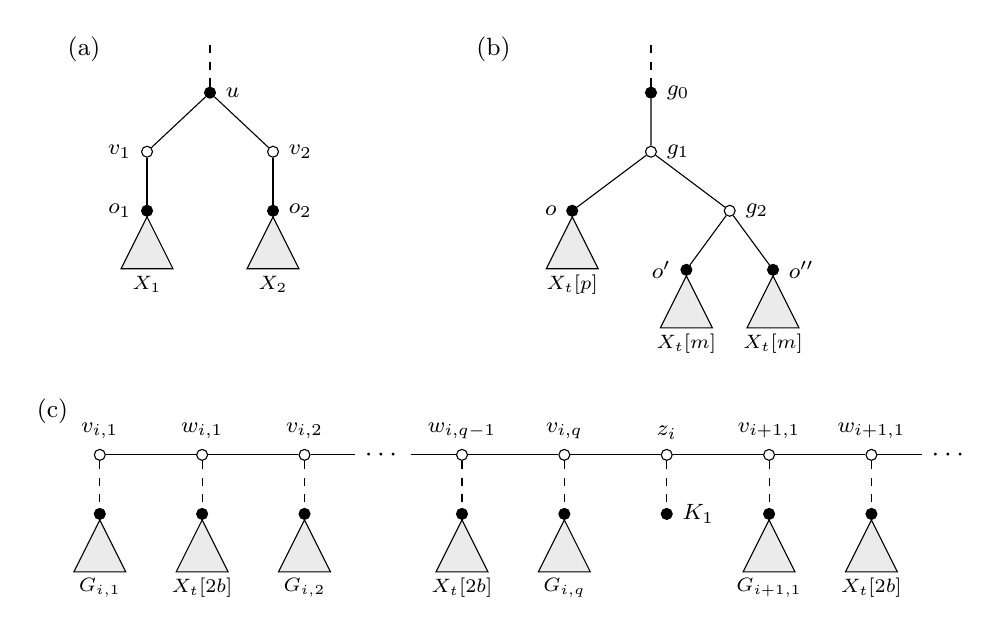
\begin{tikzpicture}[
  sk/.style={circle,draw,fill=white,inner sep=1.4pt},
  rt/.style={circle,draw,fill=black,inner sep=1.4pt},
  lab/.style={font=\footnotesize},
  tri/.style={draw,fill=black!8}]
\newcommand{\blk}[2]{\draw[tri] (#1.south) -- ++(-0.33,-0.66) -- ++(0.66,0) -- cycle; \node[font=\scriptsize] at ($(#1.south)+(0,-0.86)$) {#2};}
\begin{scope}
\node[font=\small] at (-1.6,0.55) {(a)};
\node[rt,label={[lab]right:$u$}] (u) at (0,0) {};
\draw[dashed] (u) -- ++(0,0.6);
\node[sk,label={[lab]left:$v_1$}] (v1) at (-0.8,-0.75) {};
\node[sk,label={[lab]right:$v_2$}] (v2) at (0.8,-0.75) {};
\node[rt,label={[lab]left:$o_1$}] (o1) at (-0.8,-1.5) {};
\node[rt,label={[lab]right:$o_2$}] (o2) at (0.8,-1.5) {};
\draw (v1) -- (u) -- (v2); \draw (v1) -- (o1); \draw (v2) -- (o2);
\blk{o1}{$X_1$} \blk{o2}{$X_2$}
\end{scope}
\begin{scope}[xshift=5.6cm]
\node[font=\small] at (-2.0,0.55) {(b)};
\node[rt,label={[lab]right:$g_0$}] (g0) at (0,0) {};
\draw[dashed] (g0) -- ++(0,0.6);
\node[sk,label={[lab]right:$g_1$}] (g1) at (0,-0.75) {};
\node[rt,label={[lab]left:$o$}] (o) at (-1.0,-1.5) {};
\node[sk,label={[lab]right:$g_2$}] (g2) at (1.0,-1.5) {};
\node[rt,label={[lab]left:$o'$}] (op) at (0.45,-2.25) {};
\node[rt,label={[lab]right:$o''$}] (opp) at (1.55,-2.25) {};
\draw (g0) -- (g1) -- (o); \draw (g1) -- (g2); \draw (g2) -- (op); \draw (g2) -- (opp);
\blk{o}{$X_t[p]$} \blk{op}{$X_t[m]$} \blk{opp}{$X_t[m]$}
\end{scope}
\begin{scope}[yshift=-4.6cm,xshift=-1.4cm]
\node[font=\small] at (-0.6,0.55) {(c)};
\node[sk,label={[lab]above:$v_{i,1}$}] (a1) at (0,0) {};
\node[sk,label={[lab]above:$w_{i,1}$}] (a2) at (1.3,0) {};
\node[sk,label={[lab]above:$v_{i,2}$}] (a3) at (2.6,0) {};
\node (d1) at (3.6,0) {$\cdots$};
\node[sk,label={[lab]above:$w_{i,q-1}$}] (a4) at (4.6,0) {};
\node[sk,label={[lab]above:$v_{i,q}$}] (a5) at (5.9,0) {};
\node[sk,label={[lab]above:$z_i$}] (zb) at (7.2,0) {};
\node[sk,label={[lab]above:$v_{i+1,1}$}] (b1) at (8.5,0) {};
\node[sk,label={[lab]above:$w_{i+1,1}$}] (b2) at (9.8,0) {};
\node (d2) at (10.8,0) {$\cdots$};
\draw (a1) -- (a2) -- (a3) -- (d1) -- (a4) -- (a5) -- (zb) -- (b1) -- (b2) -- (d2);
\foreach \s/\n in {a1/G_{i,1},a3/G_{i,2},a5/G_{i,q},b1/G_{i+1,1}} {
  \node[rt] (r\s) at ($(\s)+(0,-0.75)$) {}; \draw[dashed] (\s) -- (r\s); \blk{r\s}{$\n$}}
\foreach \s in {a2,a4,b2} {
  \node[rt] (r\s) at ($(\s)+(0,-0.75)$) {}; \draw[dashed] (\s) -- (r\s); \blk{r\s}{$X_t[2b]$}}
\node[rt,label={[lab]right:$K_1$}] (lf) at ($(zb)+(0,-0.75)$) {}; \draw[dashed] (zb) -- (lf);
\end{scope}
\end{tikzpicture}
\caption{(a) The product $X_1\cs X_2$ of Definition~\ref{def:product}. (b) The interface block $G_t[p,m]$ of Definition~\ref{def:interface}. (c) Part of the tree $T(r,H)$ of Definition~\ref{def:T}: the chain $C_i$, the bridge $z_i$ with its leaf, and the beginning of $C_{i+1}$; here $G_{i,k}=G_t[p_{i,k},m_i]$. Skeleton vertices are white and roots of blocks are black. A triangle is a rooted block whose root, at its apex, has degree at most two inside the block. A dashed edge joins the root of a block to the vertex at which the block is attached.}
\label{fig:construction}
\end{figure}

For a skeleton vertex $y$ we write $(A_y,B_y)$ for $(A_X,B_X)$, where $X$ is the block attached at $y$.

\begin{lemma}\label{lem:T}
The graph $T$ is a tree of maximum degree at most three. With
\begin{equation}\label{eq:S}
S=16q^4-7q^3+q^2+\sigma,
\end{equation}
we have $S<16q^4$,
\begin{equation}\label{eq:size}
|V(T)|=4\ell S-7q^2+4q-2,\qquad\alpha(T)=2\ell S-3q^2+2q-1=\frac{|V(T)|+q^2}2,
\end{equation}
and
\begin{equation}\label{eq:RT}
\R I(T)=\sum_{U\in\cI(\Gamma)}\ \prod_{y\in U}B_y\prod_{y\in V(\Gamma)\setminus U}A_y.
\end{equation}
\end{lemma}

\begin{proof}
The skeleton is a tree, and each block is attached by a single edge, so $T$ is a tree. In $\Gamma$ an inner site has two neighbours, an end site $v_{i,1}$ or $v_{i,q}$ has one coupler and at most one bridge as neighbours, and couplers and bridges have two neighbours. Each skeleton vertex receives one block, so it has degree at most three in $T$. The roots of the blocks $G_t[\cdot,\cdot]$, $X_t[\cdot]$ and $K_1$ have degree one, two and zero inside their blocks, hence degree at most three in $T$, and the remaining vertices have degree at most three by Lemmas~\ref{lem:blocks} and~\ref{lem:interface}.

Every block is gap-one with $A(0)=1$, so Corollary~\ref{cor:weights}(b) applies at each skeleton vertex. The term $U=\emptyset$ of~\eqref{eq:statesum} has constant term $1$, and Lemma~\ref{lem:statesum} gives~\eqref{eq:RT} together with $\alpha(T)=\sum_X\alpha(X)$, the sum running over all attached blocks.

For the counts we list the copies of blocks $X_t[\cdot]$. Each site contributes one copy of $X_t[p_{i,k}]$ and two copies of $X_t[m_i]$, and each coupler one copy of $X_t[2b]$, so there are $3q^2+q(q-1)=4q^2-q$ copies. The sum of their parameters is
\[
\sum_{i=1}^q\Bigl(b\sum_{k=1}^qe_k+i^2\Bigr)+2bq(q-1)+2q\sum_{i=1}^q(M+i)=8q^3(q-1)+\sigma+8q^4+q^3+q^2=S,
\]
using $\sum_ke_k=2(q-1)$. Since $\sigma\le q^3$, we have $S\le16q^4-6q^3+q^2<16q^4$. Besides these copies, $T$ contains three vertices $g_0,g_1,g_2$ per site, the $q(2q-1)$ vertices of the chains, the $q-1$ bridges and their $q-1$ leaves, that is, $5q^2+q-2$ vertices. By Lemma~\ref{lem:blocks}, $|V(T)|=4\ell S-3(4q^2-q)+5q^2+q-2$. For $\alpha(T)$, each copy of $X_t[p]$ contributes $2\ell p-1$, each interface block one more, and each leaf one, so $\alpha(T)=2\ell S-(4q^2-q)+q^2+(q-1)$.
\end{proof}

By~\eqref{eq:RT} the reversed polynomial of $T$ is a sum over the states of the skeleton with weights normalized at the common degree $\alpha(T)$. For a family $\varphi=(\varphi^0_y,\varphi^1_y)_{y\in V(C_i)}$ of power series with nonnegative coefficients we write
\[
Z_i[\varphi]=\sum_{U\in\cI(C_i)}\ \prod_{y\in U}\varphi^1_y\prod_{y\in V(C_i)\setminus U}\varphi^0_y
\]
for the corresponding chain sum, and $Z_i^{\mathrm{ex}}=Z_i[(A_y,B_y)]$ for the exact one. If $\varphi_y^\epsilon\preceq\psi_y^\epsilon$ for all $y$ and $\epsilon$, then $Z_i[\varphi]\preceq Z_i[\psi]$.

\section{The comparison model}\label{sec:gauss}

\begin{lemma}\label{lem:gauss}
Let $q\ge2$, $a\ge256$ and $\lambda>0$, and let
\[
F_\lambda(x)=\prod_{i=1}^q\Bigl(a^{i^2}+\bigl(1+\lambda a^{2i}x\bigr)^q\Bigr),\qquad\gamma_j=\binom qj\lambda^ja^{\sigma+j^2}.
\]
Then $\gamma_j\le\coef{j}{F_\lambda}\le3\gamma_j$ for $0\le j\le q$.
\end{lemma}

\begin{proof}
All coefficients of the factors are nonnegative. For $j\ge1$ take the term of degree $j$ of the factor $i=j$ and the constants $a^{i^2}$ of the other factors; this gives $\binom qj\lambda^ja^{2j^2}\cdot a^{\sigma-j^2}=\gamma_j$. For $j=0$, $\coef0{F_\lambda}=\prod_i(a^{i^2}+1)\ge a^\sigma$.

For the upper bound put
\[
\varpi=\prod_{i\ge1}\bigl(1+a^{-i^2}\bigr)\le e^{2/a}<\tfrac32,\qquad\theta=\sum_{n\in\mathbb Z}a^{-n^2}\le1+\tfrac4a<\tfrac32.
\]
The case $j=0$ follows from $\coef0{F_\lambda}=a^\sigma\prod_{i\le q}(1+a^{-i^2})\le\varpi\gamma_0$. Let $j\ge1$. A contribution to $\coef j{F_\lambda}$ is determined by a nonempty set $\cA\subseteq\{1,\dots,q\}$ of \emph{active} factors and degrees $u_i\ge1$ $(i\in\cA)$ with $\sum_{i\in\cA}u_i=j$; it equals
\[
\prod_{i\in\cA}\binom q{u_i}\lambda^{u_i}a^{2iu_i}\prod_{i\notin\cA}\bigl(a^{i^2}+1\bigr).
\]
Using $2iu-i^2=u^2-(i-u)^2$, its ratio to $\gamma_j$ is at most
\begin{equation}\label{eq:gauss-ratio}
\varpi\binom qj^{-1}\prod_{i\in\cA}\binom q{u_i}\cdot a^{\sum_{i\in\cA}u_i^2-j^2}\prod_{i\in\cA}a^{-(i-u_i)^2}.
\end{equation}
Let $k=|\cA|$. Since all $u_i\ge1$, $\sum u_i^2\le(j-k+1)^2+(k-1)$, hence $j^2-\sum u_i^2\ge(k-1)(2j-k)\ge(k-1)j$.

If $k=1$, then $\cA=\{i\}$ with $u_i=j$, and the sum of~\eqref{eq:gauss-ratio} over $i$ is at most $\varpi\theta$.

If $k\ge2$, sum over ordered $k$-tuples of distinct indices and divide by $k!$. Extending each index to all of $\mathbb Z$ and using Vandermonde's identity $\sum\prod_h\binom q{u_h}\le\binom{kq}j$, the total contribution of all $\cA$ with $|\cA|=k$ is at most
\[
\varpi\,\frac{\theta^k}{k!}\,a^{-(k-1)j}\binom{kq}j\binom qj^{-1}\le\varpi\,\frac{\theta^k}{k!}\Bigl(\frac{3k}{a^{k-1}}\Bigr)^j,
\]
where $\binom{kq}j\le(ekq/j)^j$ and $\binom qj\ge(q/j)^j$ were used. Since $3k\le8^{k-1}$ and $a\ge256$, we have $3k/a^{k-1}\le32^{-(k-1)}\le1$, so the last expression is at most $\varpi\,2^k32^{-(k-1)}$. Summing over $k\ge2$ gives at most $\varpi\cdot\frac2{15}$. Altogether $\coef j{F_\lambda}\le\varpi(\theta+\tfrac2{15})\gamma_j\le\tfrac32\cdot\tfrac{49}{30}\gamma_j=\tfrac{49}{20}\gamma_j<3\gamma_j$.
\end{proof}

We apply the lemma with $\lambda=a^{2M}$. Put
\begin{equation}\label{eq:L}
\kappa_0=a^{2b(q-1)},\qquad \kappa=\kappa_0^q,\qquad P_i=1+a^{2m_i}x,\qquad F=\prod_{i=1}^q\bigl(a^{i^2}+P_i^q\bigr),
\end{equation}
and
\[
L_j=\kappa\binom qja^{\sigma+2Mj+j^2}\qquad(0\le j\le q).
\]
Since $P_i=1+a^{2M}a^{2i}x$, Lemma~\ref{lem:gauss} gives
\begin{equation}\label{eq:KF}
L_j\le\coef j{(\kappa F)}\le3L_j\qquad(0\le j\le q),
\end{equation}
because $a\ge Q\ge256$.

\section{The lower bound}\label{sec:lower}

The \emph{lower model} $\varphi^-$ on $C_i$ assigns the weights
\[
\varphi^-_{v_{i,k}}=\bigl(P_i,\ P_i+a^{p_{i,k}}\bigr),\qquad\varphi^-_{w_{i,k}}=\bigl(1,\ a^{2b}\bigr).
\]

\begin{lemma}\label{lem:lower-weights}
For every site and coupler of $C_i$ we have $\varphi^{-,\epsilon}_y\preceq(A_y,B_y)^\epsilon$ for $\epsilon=0,1$. Hence $Z_i[\varphi^-]\preceq Z_i^{\mathrm{ex}}$.
\end{lemma}

\begin{proof}
Let $y=v_{i,k}$, $p=p_{i,k}$ and $m=m_i$, and use the notation of Lemma~\ref{lem:interface}. By Lemma~\ref{lem:envelope} and~\eqref{eq:entropy}, $A_p\succeq1$, $A_m\succeq1$, $B_m\succeq d_m^\ast\ge a^m$ and $B_p\succeq d_p^\ast\ge a^p$. Hence $E\succeq1+(d_m^\ast)^2x\succeq P_i$ and $O\succeq a^p$, so $A_y=E+x(E+O)\succeq P_i$ and $B_y=E+O\succeq P_i+a^p$. For a coupler, $A_{2b}\succeq1$ and $B_{2b}\succeq d^\ast_{2b}\ge a^{2b}$.
\end{proof}

The next lemma compares the configurations of a single chain.

\begin{lemma}\label{lem:phase}
Let $F_i=a^{i^2}+P_i^q$ and $\varepsilon=2qa^{-4q^2}+2\cdot3^qa^{-q^2}$. Then
\[
\kappa_0F_i\preceq Z_i[\varphi^-]\preceq(1+\varepsilon)\kappa_0F_i,
\]
and $q\varepsilon<\frac14$.
\end{lemma}

\begin{proof}
Write $v_k=v_{i,k}$, $w_k=w_{i,k}$ and $p_k=p_{i,k}$. The sites of $C_i$ are pairwise nonadjacent, so any set $U\subseteq\{1,\dots,q\}$ of selected sites is allowed, and the coupler $w_k$ may be selected exactly when $k,k+1\notin U$. Let $e_{00}(U)$ be the number of $k\in\{1,\dots,q-1\}$ with $k,k+1\notin U$, and $\mathrm{cut}(U)$ the number of $k$ with exactly one of $k,k+1$ in $U$. Summing over couplers and expanding each selected site weight $P_i+a^{p_k}$ according to the set $\Phi\subseteq U$ of sites taking the constant summand,
\[
Z_i[\varphi^-]=\sum_{\Phi\subseteq U\subseteq\{1,\dots,q\}}a^{\sum_{k\in\Phi}p_k}\bigl(1+a^{2b}\bigr)^{e_{00}(U)}P_i^{\,q-|\Phi|}.
\]
Counting the endpoints of the $q-1$ edges $\{k,k+1\}$ gives $\sum_{k\in U}e_k+2e_{00}(U)=2(q-1)-\mathrm{cut}(U)$. Together with $\sum_{k\in\Phi}p_k=b\sum_{k\in U}e_k+i^2[1\in U]-\sum_{k\in U\setminus\Phi}p_k$, this shows that the term of $(U,\Phi)$ equals $\kappa_0$ times
\begin{equation}\label{eq:phase-term}
a^{\,i^2[1\in U]-b\,\mathrm{cut}(U)-\sum_{k\in U\setminus\Phi}p_k}\bigl(1+a^{-2b}\bigr)^{e_{00}(U)}P_i^{\,q-|\Phi|}.
\end{equation}
The pair $U=\Phi=\emptyset$ gives $(1+a^{-2b})^{q-1}P_i^q$, and $U=\Phi=\{1,\dots,q\}$ gives $a^{i^2}$. This proves the lower bound. For every other pair, either $\emptyset\ne U\ne\{1,\dots,q\}$, and then $\mathrm{cut}(U)\ge1$, or $U=\{1,\dots,q\}\ne\Phi$, and then $\sum_{U\setminus\Phi}p_k\ge b$. In both cases the exponent in~\eqref{eq:phase-term} is at most $i^2-b\le q^2-2q^2=-q^2$. There are $3^q$ pairs, and $P_i^{q-|\Phi|}\preceq P_i^q$. Put $u=(q-1)a^{-2b}=(q-1)a^{-4q^2}\le\frac12$. Since $e^u-1\le2u$ for $0\le u\le1$,
\[
\bigl(1+a^{-2b}\bigr)^{q-1}-1\le e^u-1\le2qa^{-4q^2},\qquad\bigl(1+a^{-2b}\bigr)^{q-1}\le e^{1/2}<2,
\]
and therefore
\[
Z_i[\varphi^-]\preceq\kappa_0\Bigl(a^{i^2}+P_i^q+\bigl(2qa^{-4q^2}+2\cdot3^qa^{-q^2}\bigr)P_i^q\Bigr)\preceq(1+\varepsilon)\kappa_0F_i.
\]
Finally $q\varepsilon=2q^2a^{-4q^2}+2q3^qa^{-q^2}$ decreases in $q\ge2$ for $a\ge256$, so $q\varepsilon\le8a^{-16}+36a^{-4}<\frac14$.
\end{proof}

\begin{proposition}\label{prop:lower}
For $0\le j\le q$ we have $c_j(T)\ge L_j$. Moreover
\begin{equation}\label{eq:model-product}
\kappa F\preceq\prod_{i=1}^qZ_i[\varphi^-]\preceq2\kappa F.
\end{equation}
\end{proposition}

\begin{proof}
By Lemma~\ref{lem:phase}, $\prod_iZ_i[\varphi^-]\preceq(1+\varepsilon)^q\kappa F$ and $(1+\varepsilon)^q\le e^{q\varepsilon}<e^{1/4}<2$, which gives~\eqref{eq:model-product}. In~\eqref{eq:RT} keep only the sets $U$ containing no bridge. A bridge $z_i\notin U$ has weight $A_{K_1}=1+x$ and imposes no restriction on its neighbours, so these terms add up to $(1+x)^{q-1}\prod_iZ_i^{\mathrm{ex}}$. By Lemma~\ref{lem:lower-weights} and~\eqref{eq:model-product},
\[
\R I(T)\succeq(1+x)^{q-1}\prod_{i=1}^qZ_i^{\mathrm{ex}}\succeq\prod_{i=1}^qZ_i[\varphi^-]\succeq\kappa F,
\]
and~\eqref{eq:KF} gives $c_j(T)\ge L_j$.
\end{proof}

\section{The upper bound}\label{sec:upper}

We first record the size of the parameters. By Lemma~\ref{lem:blocks}(i) and the minimality of $t$,
\begin{equation}\label{eq:a-size}
Q\le a\le Q^2,\qquad\ell\le\log_2a,
\end{equation}
since $d_{t-1}\le Q-1$ gives $a=(1+d_{t-1})^2\le Q^2$, and $a\ge2^{2^t}=2^\ell$. In particular $a\ge2^{12}q^4\ge128q^4$. Every block parameter $p$ occurring in $T$ satisfies $p\le M+q$: indeed $p_{i,k}\le\max(b+q^2,2b)=4q^2$, $2b=4q^2$ and $m_i\le M+q$. As $2(M+q)/a<\frac12$, the bound~\eqref{eq:entropy} gives
\begin{equation}\label{eq:d-small}
d_p^\ast\le2a^p\le2a^{M+q}\qquad\text{for all parameters }p\text{ occurring in }T.
\end{equation}

\begin{lemma}\label{lem:site-envelope}
Let $G=G_t[p,m]$ and put $\bar P=1+(d_m^\ast)^2x$ and
\[
R_G=\frac1{(1-\omega_px)(1-\omega_mx)^2(1-(1+d^\ast_p)x)}.
\]
Then $A_G\preceq R_G\bar P$ and $B_G\preceq R_G\,(\bar P+d^\ast_p)$.
\end{lemma}

\begin{proof}
Put $R_0=(1-\omega_px)^{-1}(1-\omega_mx)^{-2}$. By~\eqref{eq:block-envelope},
\[
E=A_p\bigl(A_m^2+xB_m^2\bigr)\preceq R_0\bigl(1+(d_m^\ast)^2x\bigr)=R_0\bar P,\qquad O=B_pA_m^2\preceq R_0d^\ast_p.
\]
Hence $B_G=E+O\preceq R_0(\bar P+d^\ast_p)\preceq R_G(\bar P+d_p^\ast)$. Moreover
\[
A_G=E+x(E+O)\preceq R_0\bigl(\bar P+x(\bar P+d_p^\ast)\bigr)\preceq R_0\bar P\bigl(1+(1+d^\ast_p)x\bigr)\preceq R_G\bar P,
\]
where we used $d^\ast_px\preceq d^\ast_px\bar P$ and $1+(1+d_p^\ast)x\preceq(1-(1+d_p^\ast)x)^{-1}$.
\end{proof}

The \emph{upper model} $\varphi^+$ on $C_i$ assigns, with $\bar P_i=1+(d^\ast_{m_i})^2x$,
\[
\varphi^+_{v_{i,k}}=\bigl(\bar P_i,\ \bar P_i+d^\ast_{p_{i,k}}\bigr),\qquad\varphi^+_{w_{i,k}}=\bigl(1,\ d^\ast_{2b}\bigr).
\]
It has the same shape as $\varphi^-$, with $a^p$ replaced by $d^\ast_p$.

\begin{lemma}\label{lem:models}
We have $\prod_{i=1}^qZ_i[\varphi^+]\preceq2\prod_{i=1}^qZ_i[\varphi^-]\pmod{x^{q+1}}$.
\end{lemma}

\begin{proof}
Expand both products as in the proof of Lemma~\ref{lem:phase}, now over all chains simultaneously and including the selected couplers: a term is indexed by independent sets $U_i\in\cI(C_i)$ together with sets $\Phi_i$ of selected sites taking the constant summand. Let $n_i$ be the number of sites of $C_i$ not in $\Phi_i$. The term of $\varphi^+$ is $\prod d^\ast_p\cdot\prod_i\bar P_i^{n_i}$, the first product running over the constants used, namely the sites in some $\Phi_i$ and the selected couplers; the term of $\varphi^-$ is $\prod a^p\cdot\prod_iP_i^{n_i}$ with the same indices. Each site and each coupler occurs at most once, so the sum of the parameters $p$ involved is at most
\[
\sum_{i,k}p_{i,k}+2bq(q-1)=4bq(q-1)+\sigma\le8q^4,
\]
and~\eqref{eq:entropy} gives $\prod d^\ast_p\le e^{16q^4/a}\prod a^p$. Next, $(d^\ast_{m_i})^2\le a^{2m_i}e^{4(M+q)/a}$, so that for every $n$
\[
\coef n{\prod_i\bar P_i^{n_i}}=\sum_{n_1'+\dots+n_q'=n}\ \prod_i\binom{n_i}{n_i'}(d^\ast_{m_i})^{2n_i'}\le e^{4(M+q)n/a}\coef n{\prod_iP_i^{n_i}}.
\]
For $n\le q$ the coefficients of degree $n$ of corresponding terms therefore differ by at most the factor $\exp\bigl((16q^4+4q(M+q))/a\bigr)\le e^{26q^4/a}\le e^{26/128}<2$, where $16q^3+4q^2\le10q^4$ for $q\ge2$ and $a\ge128q^4$ were used. Summing over all terms proves the lemma.
\end{proof}

\begin{proposition}\label{prop:upper}
For $0\le j\le q$ we have $c_j(T)\le2^{q+3}L_j$.
\end{proposition}

\begin{proof}
\emph{Bridges.} The bridges are pairwise nonadjacent. Group the terms of~\eqref{eq:RT} according to the set of selected bridges, and drop the condition that the end sites next to a selected bridge are unselected; this can only increase the coefficients. Since $A_{K_1}+B_{K_1}=2+x\preceq2(1-x)^{-1}$,
\[
\R I(T)\preceq(2+x)^{q-1}\prod_{i=1}^qZ_i^{\mathrm{ex}}\preceq\frac{2^{q-1}}{(1-x)^{q-1}}\prod_{i=1}^qZ_i^{\mathrm{ex}}.
\]

\emph{Common envelopes.} For a site $y$ with block $G$ let $R_y=R_G$ (Lemma~\ref{lem:site-envelope}), and for a coupler let $R_y=(1-\omega_{2b}x)^{-1}$. By Lemmas~\ref{lem:envelope} and~\ref{lem:site-envelope}, $(A_y,B_y)^\epsilon\preceq R_y\,\varphi^{+,\epsilon}_y$ for $\epsilon=0,1$, with the same factor $R_y$ in both states. Since every term of a chain sum contains exactly one weight of each vertex, $Z_i^{\mathrm{ex}}\preceq\bigl(\prod_{y\in V(C_i)}R_y\bigr)Z_i[\varphi^+]$. Put
\[
\mathcal R=\frac1{(1-x)^{q-1}}\prod_{i=1}^q\prod_{y\in V(C_i)}R_y.
\]
By Lemma~\ref{lem:models} and~\eqref{eq:model-product},
\begin{equation}\label{eq:upper-chain}
\R I(T)\preceq2^{q-1}\,\mathcal R\cdot2\prod_iZ_i[\varphi^-]\preceq2^{q+1}\,\mathcal R\,\kappa F\pmod{x^{q+1}}.
\end{equation}

\emph{The envelope $\mathcal R$.} The series $\mathcal R$ is a product of factors of the form $(1-\lambda x)^{-1}$: one for each copy of a block $X_t[p]$ in $T$, with $\lambda=\omega_p$; one for each site $v_{i,k}$, with $\lambda=1+d^\ast_{p_{i,k}}$; and $q-1$ further factors with $\lambda=1$. By~\eqref{eq:envelope-basic}, $\coef k{\mathcal R}\le W^k$, where $W$ denotes the sum of all these $\lambda$. By Lemma~\ref{lem:envelope}, Lemma~\ref{lem:blocks}, \eqref{eq:d-small} and~\eqref{eq:a-size},
\[
\omega_p\le|X_t[p]|\,d^\ast_p\le4\ell p\cdot2a^{M+q},
\]
and the parameters of all copies sum to $S<16q^4$, so these copies contribute at most
\[
128q^4\ell a^{M+q}\le128q^4\log_2(a)\,a^{M+q}.
\]
The $q^2$ sites contribute at most $3q^2a^{M+q}$ and the bridges $q-1\le q^2a^{M+q}$. Hence
\[
W\le132\,q^4\log_2(a)\,a^{M+q}.
\]

\emph{Conclusion.} For $1\le j\le q$,
\[
\frac{L_{j-1}}{L_j}=\frac{j}{q-j+1}\,a^{-2M-2j+1}\le\frac q{a^{2M}},
\]
so $L_{j-k}\le(q/a^{2M})^kL_j$ for $0\le k\le j$. Using $\log_2a\le a$, $M=4q^2$ and the monotonicity in $q\ge2$,
\[
\frac{qW}{a^{2M}}\le132\,q^5a^{-(4q^2-q-1)}\le4224\,a^{-13}<\frac14.
\]
By~\eqref{eq:upper-chain} and~\eqref{eq:KF}, for $0\le j\le q$,
\[
c_j(T)\le2^{q+1}\sum_{k=0}^jW^k\coef{j-k}{(\kappa F)}\le3\cdot2^{q+1}\sum_{k=0}^jW^kL_{j-k}\le3\cdot2^{q+1}L_j\sum_{k\ge0}4^{-k}=2^{q+3}L_j.\qedhere
\]
\end{proof}

\section{Proof of the main theorem}\label{sec:proof}

\begin{theorem}\label{thm:two-sided}
Let $r,H\ge1$, $q=r+1$, and let $T=T(r,H)$ be as in Definition~\ref{def:T}. Then
\[
L_j\le c_j(T)\le2^{q+3}L_j\qquad(0\le j\le q),\qquad L_j=a^{2bq(q-1)}\binom qja^{\sigma+2Mj+j^2}.
\]
\end{theorem}

\begin{proof}
Combine Propositions~\ref{prop:lower} and~\ref{prop:upper}.
\end{proof}

\begin{proof}[Proof of Theorem~\ref{thm:main}]
Let $T=T(r,H)$. By Lemma~\ref{lem:T} it is a tree of maximum degree at most three. For $1\le j\le q-1=r$,
\[
\frac{L_{j-1}L_{j+1}}{L_j^2}=\frac{j(q-j)}{(j+1)(q-j+1)}\,a^{(j-1)^2+(j+1)^2-2j^2}\ge\frac{a^2}4,
\]
so Theorem~\ref{thm:two-sided} and $a\ge Q=2^{q+10}q^4H$ give
\[
\frac{c_{j-1}(T)\,c_{j+1}(T)}{c_j(T)^2}\ge\frac{L_{j-1}L_{j+1}}{(2^{q+3}L_j)^2}\ge\frac{a^2}{2^{2q+8}}\ge2^{12}q^8H^2>H.
\]
As $c_j(T)=s_{\alpha-j}(T)$, this is~\eqref{eq:main}.

For the order, \eqref{eq:size}, $S<16q^4$ and~\eqref{eq:a-size} give
\[
|V(T)|<4\ell S<64q^4\log_2a\le128q^4\log_2Q.
\]
Here $\log_2Q=q+10+4\log_2q+\log_2H\le8q+\log_2H$ for $q\ge2$, and $\log_2H\le h$. Hence
\[
|V(T)|<1024\,q^5+128\,q^4h\le1200\,q^4(q+h).\qedhere
\]
\end{proof}

\begin{remark}[Construction]\label{rem:complexity}
The number $Q$ has $O(q+\log H)$ bits. The integers $d_0,d_1,\dots$ are computed by $d\mapsto(1+d)^2$ until $d\ge Q$; by~\eqref{eq:a-size} this takes $t\le\log_2\log_2a\le\log_2(2\log_2Q)$ steps on integers of at most $2\log_2Q+1$ bits. All other parameters are explicit integers, and the blocks $X_t[p]$, $G_t[p,m]$ and the tree $T$ are then written down in time linear in $|V(T)|=O(q^4(q+h))$. Thus $T(r,H)$ can be written down in time polynomial in $r$ and $\log(H+1)$. The first $q+1$ reversed coefficients of $T$ can be computed exactly by a dynamic program over the tree that keeps, for every vertex, only the coefficients of degree at most $q$ below the maximum; all integers involved have at most $|V(T)|+1$ bits.
\end{remark}

\begin{remark}[Exact computations]\label{rem:computation}
For $(r,H)\in\{(1,1),(2,1),(3,1),(4,1),(1,10^6),(2,10^6)\}$ we constructed $T(r,H)$ explicitly as adjacency lists, with $13{,}354$, $144{,}587$, $472{,}734$, $1{,}178{,}083$, $26{,}730$ and $289{,}227$ vertices respectively, and computed $c_0(T),\dots,c_q(T)$ exactly by a generic dynamic program over the tree. In every case the order, the independence number~\eqref{eq:size}, the maximum degree, the bounds of Theorem~\ref{thm:two-sided} and the inequalities~\eqref{eq:main} were confirmed. For $(r,H)=(1,1)$, for instance, $a=458{,}329$, and an exact comparison of integers gives $2^{35}<c_0c_2/c_1^2<2^{36}$; this ratio differs from the model value $L_0L_2/L_1^2=a^2/4$ by a relative amount less than $10^{-5}$. A Python script that constructs $T(r,H)$ and checks these statements with exact integer arithmetic is provided as an ancillary file. These computations are not used in the proofs.
\end{remark}

\section{Further remarks}\label{sec:remarks}

\subsection{A lower bound on the order}
The next proposition shows that, for fixed $r$, the term $q^4h$ in Theorem~\ref{thm:main} cannot be replaced by $o(\log H)$.

\begin{proposition}\label{prop:lower-order}
Let $G$ be a graph on $n$ vertices with $\alpha(G)\ge q$, where $q\ge2$, and let $H>1$. If $c_{j-1}(G)c_{j+1}(G)>H\,c_j(G)^2$ for $1\le j\le q-1$, then
\[
n>\frac12\Bigl\lfloor\frac{q^2}4\Bigr\rfloor\log_2H.
\]
\end{proposition}

\begin{proof}
Put $f_j=\log_2c_j(G)$ and $\lambda=\log_2H>0$. Since $1\le c_j(G)\le\binom n{\alpha(G)-j}<2^n$, we have $0\le f_j<n$ for $0\le j\le q$. The sequence $g_j=f_j-\lambda j^2/2$ has positive second differences on $\{0,\dots,q\}$, so it lies strictly below its chord: for $0<j<q$,
\[
f_j-\frac{\lambda j^2}2<\frac{(q-j)f_0+j\bigl(f_q-\lambda q^2/2\bigr)}q,\quad\text{that is,}\quad f_j<\frac{(q-j)f_0+jf_q}q-\frac\lambda2j(q-j).
\]
With $f_0,f_q<n$ and $f_j\ge0$ this gives $n>\frac\lambda2j(q-j)$, and $j=\lfloor q/2\rfloor$ gives the claim.
\end{proof}

With $q=r+1$, Proposition~\ref{prop:lower-order} and Theorem~\ref{thm:main} show that the least order of a graph, or of a subcubic tree, satisfying~\eqref{eq:main} lies between $C_1r^2\log H$ and $C_2(r^5+r^4\log H)$ for $H\ge2$, with absolute constants $C_1,C_2>0$. We do not know the correct exponent of $r$. For trees without restrictions on the degree or on the position of the run, Yu's construction~\cite[Corollary~1.3]{Yu} gives runs of length $r$ with $O(r^3)$ vertices; it would be interesting to know whether terminal runs of strength $H$ in subcubic trees can be obtained with $O(r^3\log(H+1))$ vertices.

\subsection{Unimodality}\label{sec:unimodality}
Levit and Mandrescu~\cite{LM} showed that the independent set sequence of a tree $T$ is decreasing from $\lceil(2\alpha(T)-1)/3\rceil$ on; see also~\cite[Section~3]{Gal}. In $T(r,H)$ the failures occur at the positions $\alpha-1,\dots,\alpha-r$, which lie in this range because $\alpha(T)>3r$. They therefore give no information on the question of Alavi, Malde, Schwenk and Erd\H{o}s~\cite{AMSE}, nor on Galvin's question~\cite[Question~3.1]{Gal} whether log-concavity can fail at distance proportional to $\alpha(T)$ from $\alpha(T)$.

\subsection{Stable-path trees}
The stable-path trees of Bencs~\cite[Definition~2.2 and Theorem~2.3]{Bencs} replace a graph by a tree with the same rooted ratio $I(G-u)/I(G)$; for a tree $G$ the construction returns $G$ itself, so it does not lower the maximum degree of earlier examples. Here the large multiplicities are produced instead by the subcubic recursion $\cs$ of Section~\ref{sec:amplifier}, at the cost of a factor $O(\log a)$ in the order.

\section*{Use of AI-assisted tools}
AI-assisted tools were used in the research and preparation of this manuscript.

\begin{thebibliography}{99}

\bibitem{AMSE}
Y.~Alavi, P.~J. Malde, A.~J. Schwenk, and P.~Erd\H{o}s, \emph{The vertex independence sequence of a graph is not constrained}, Congr. Numer. \textbf{58} (1987), 15--23.

\bibitem{BR1}
C.~Bautista-Ramos, \emph{Multiple breaks of log-concavity in the independence polynomials of trees}, preprint (2025), arXiv:2511.00334v1.

\bibitem{BR2}
C.~Bautista-Ramos, \emph{Unbounded log-concavity breaks in independence polynomials of spherically symmetric trees}, preprint (2026), arXiv:2610.04172v1.

\bibitem{BGG}
C.~Bautista-Ramos, C.~Guill\'en-Galv\'an, and P.~G\'omez-Salgado, \emph{Linear recurrences for non-log-concave independence polynomials of trees}, Graphs Combin. \textbf{42} (2026), Paper No.~59, doi:10.1007/s00373-026-03054-4. Statement numbers in the text refer to the preprint version, arXiv:2603.14204v1.

\bibitem{Bencs}
F.~Bencs, \emph{On trees with real rooted independence polynomial}, Discrete Math. \textbf{341} (2018), 3321--3330. Statement numbers in the text refer to the preprint version, arXiv:1703.05409v1.

\bibitem{Gal}
D.~Galvin, \emph{Trees with non log-concave independent set sequences}, preprint (2026), arXiv:2502.10654v2.

\bibitem{HLP}
G.~H. Hardy, J.~E. Littlewood, and G.~P\'olya, \emph{Inequalities}, 2nd ed., Cambridge University Press, Cambridge, 1952.

\bibitem{KL}
O.~Kadrawi and V.~E. Levit, \emph{The independence polynomial of trees is not always log-concave starting from order 26}, Ars Math. Contemp. \textbf{25} (2025), no.~4, Paper No.~P4.03, doi:10.26493/1855-3974.3207.2ad.

\bibitem{KLYM}
O.~Kadrawi, V.~E. Levit, R.~Yosef, and M.~Mizrachi, \emph{On computing of independence polynomials of trees}, in: Recent Research in Polynomials (F.~\"Ozger, ed.), IntechOpen, 2023, doi:10.5772/intechopen.1001130.

\bibitem{LM}
V.~E. Levit and E.~Mandrescu, \emph{Partial unimodality for independence polynomials of K\"onig--Egerv\'ary graphs}, Congr. Numer. \textbf{179} (2006), 109--119.

\bibitem{WZ}
Y.~Wang and B.-X. Zhu, \emph{On the unimodality of independence polynomials of some graphs}, European J. Combin. \textbf{32} (2011), no.~1, 10--20.

\bibitem{Yu}
X.~Yu, \emph{Unbounded runs of non-log-concavity in independence polynomials of trees}, preprint (2026), included in Zenodo record 22263331, version~1.1.0, doi:10.5281/zenodo.22263331. Statement numbers in the text refer to this version. The exact records of the run of $T(2^{13}1^{13})$ quoted in Section~1 are in the file \nolinkurl{search_results/bencs_spherical_extension_probe.json} of the same record.

\end{thebibliography}

\end{document}
